\documentclass[twocolumn]{extarticle}
\usepackage{fontspec}   %加這個就可以設定字體
\usepackage{xeCJK}       %讓中英文字體分開設置
\usepackage{indentfirst}
\usepackage{listings}
\usepackage[newfloat]{minted}
\usepackage{float}
\usepackage{graphicx}
\usepackage{caption}
\usepackage{fancyhdr}
\usepackage{hyperref}
\usepackage{amsmath}
\usepackage{multirow}
\usepackage[dvipsnames]{xcolor}
\usepackage{graphicx}
\usepackage{tabularx}
\usepackage{booktabs}
\usepackage{caption}
\usepackage{subcaption}
\usepackage{pifont}
\usepackage{amssymb}
\usepackage{titling}


\usepackage{pdftexcmds}
\usepackage{catchfile}
\usepackage{ifluatex}
\usepackage{ifplatform}

\usepackage[breakable, listings, skins, minted]{tcolorbox}
\usepackage{etoolbox}
\setminted{fontsize=\footnotesize}
\renewtcblisting{minted}{%
    listing engine=minted,
    minted language=python,
    listing only,
    breakable,
    enhanced,
    minted options = {
        linenos, 
        breaklines=true, 
        breakbefore=., 
        % fontsize=\footnotesize, 
        numbersep=2mm
    },
    overlay={%
        \begin{tcbclipinterior}
            \fill[gray!25] (frame.south west) rectangle ([xshift=4mm]frame.north west);
        \end{tcbclipinterior}
    }   
}

\usepackage[
top=1.5cm,
bottom=0.75cm,
left=1.5cm,
right=1.5cm,
includehead,includefoot,
heightrounded, % to avoid spurious underfull messages
]{geometry} 

\newenvironment{code}{\captionsetup{type=listing}}{}
\SetupFloatingEnvironment{listing}{name=Code}
\usepackage[moderate]{savetrees}


\title{NYCU Introduction to Machine Learning, Homework 1}
\author{110550088 李杰穎}
\date{}


\setCJKmainfont{Noto Serif TC}


\ifwindows
\setmonofont[Mapping=tex-text]{Consolas}
\fi

\XeTeXlinebreaklocale "zh"             %這兩行一定要加,中文才能自動換行
\XeTeXlinebreakskip = 0pt plus 1pt     %這兩行一定要加,中文才能自動換行

\setlength{\parindent}{0em}
\setlength{\parskip}{2em}
\renewcommand{\baselinestretch}{1.25}
\setlength{\droptitle}{-7.5em}   % This is your set screw
\setlength{\columnsep}{2em}
\usepackage{enumitem}

\begin{document}

\maketitle

\section{Part. 1, Coding (50\%)}
\subsection{(10\%) Linear Regression Model - Closed-form Solution}
\begin{enumerate}
\item (10\%)  Show the weights and intercepts of your linear model.
\begin{figure}[H]
\centering
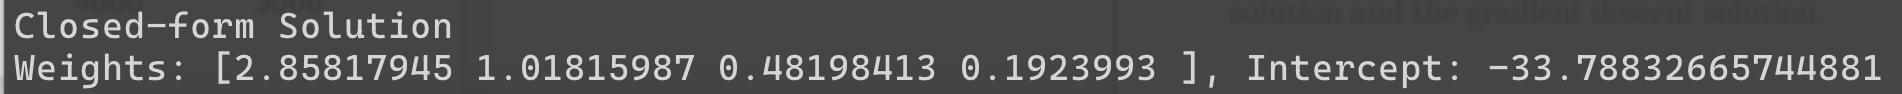
\includegraphics[width=\linewidth]{closed_form_weights}
\caption{The weights and intercepts given by closed-form solution.}
\label{fig:closedformweights}
\end{figure}


\end{enumerate}

\subsection{(40\%) Linear Regression Model - Gradient Descent Solution}

\begin{enumerate}
\setcounter{enumi}{1}
\item (0\%)   Show the learning rate and epoch (and batch size if you implement mini-batch gradient descent) you choose.
\begin{itemize}
	\item Learning rate: $2 \times 10^4$
	\item Epoch: 50
	\item Mini-batch size: 10 (with random sampling)
\end{itemize}
\item (10\%) Show the weights and intercepts of your linear model.
\begin{figure}[H]
\centering
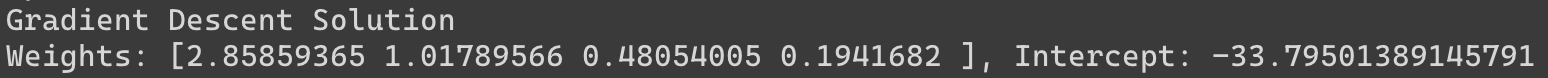
\includegraphics[width=\linewidth]{gradient_weights}
\caption{The weights and intercepts given by mini-batch gradient descent solution.}
\label{fig:gradientweights}
\end{figure}


\item (10\%) Plot the learning curve. (x-axis=epoch, y-axis=training loss)
\begin{figure}[H]
\centering
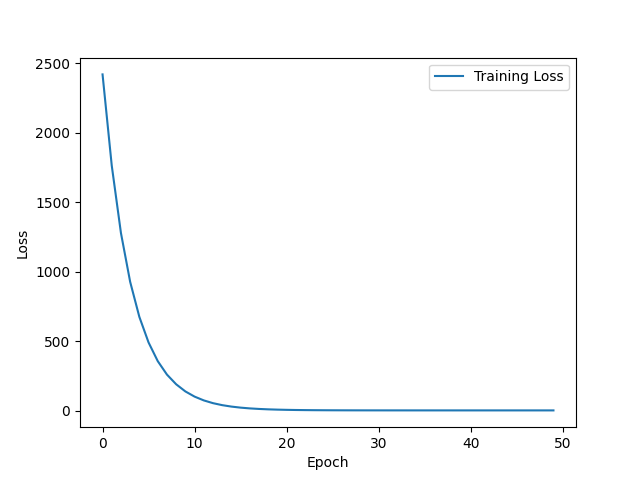
\includegraphics[width=\linewidth]{lr_plot}
\caption{The plot of training loss to epoch.}
\label{fig:lrplot}
\end{figure}

\item (20\%) Show your error rate between your closed-form solution and the gradient descent solution.
\begin{figure}[H]
\centering

\includegraphics[width=0.5\linewidth]{error_rate}
\caption{The error rate between closed-form solution and gradient descent solution.}
\label{fig:errorrate}
\end{figure}
\end{enumerate}

I think it's worth noticing that I actually normalize the training data before performing gradient descent. I found that the value of ``Previous Scores'' is much greater than other features, this will make gradient descent unstable, and will take lots of time to converge to optimal solution. Therefore, I normalized each feature by,

\begin{equation*}
X_{i}' = \frac{X_i - \mu_i}{\sigma_i}
\end{equation*}

, where $\mu_i$ is the mean of feature $i$, and $\sigma_i$ is the standard deviation of feature $i$. This is actually standardization. With this normalization, we can quickly approach optimal solution in only 50 epochs.

And because the normalization operation is linear, after we get the optimal weights $\beta'$ and intercepts $\beta_0'$ under $X'$, we can convert $\beta'$ and $\beta_0'$ back to $\beta$ and $\beta_0$ under distribution of $X$ by,

\begin{equation*}
\beta_i = \frac{\beta_i'}{\sigma_i}
\end{equation*}

and

\begin{equation*}
\beta_0 = \beta_0' - \sum_{i} \beta_i' \cdot \, \frac{\mu_i}{\sigma_i}
\end{equation*}

\section{Part. 2, Questions (50\%)}
\begin{enumerate}
\item (10\%) How does the value of learning rate impact the training process in gradient descent? Please explain in detail.

If the learning rate is too large, then it may cause gradient exploration, made the weights and intercept goes to infinity, leading to divergence. Even if the model doesn't diverge, large learning rate may cause the algorithm missed the minima of loss function, and can't converge to the optimal solution.

If the learning rate is too small, then it has greater chance to stuck in local minima, which will make us not be able to get the optimal solution. And also, small learning rate leads to longer convergence time.

\item (10\%) There are some cases where gradient descent may fail to converge. Please provide at least two scenarios and explain in detail.

\begin{itemize}
\item Linear regression is not applicable to the data: If the data can not be approximated using linear equation, then the surface of loss function may not have a significant minima. This may make gradient descent fail to converge.
\item Different scale across each feature: If the features is significantly difference in scale (or let's say, the range of value), this will make gradient descent very unstable, so that we can only use a smaller learning rate, but this will arise another problem: slow training. Therefore, normalize the data, as I've done in this homework, before apply gradient descent is very important.
\end{itemize}


\item (15\%) Is mean square error (MSE) the optimal selection when modeling a simple linear regression model? Describe why MSE is effective for resolving most linear regression problems and list scenarios where MSE may be inappropriate for data modeling, proposing alternative loss functions suitable for linear regression modeling in those cases.

Let's first talk about the advantages of using MSE as loss function:

\begin{itemize}
\item Differentiable: MSE is differentiable everywhere, therefore, we can use gradient descent method to optimize the parameters. If we're using something like L1 Loss, then it's not differentiable at $x=0$. Make it a little bit harder to perform gradient descent.
\item Least square solution: In linear algebra, we have a closed-form method to find the least square solution of a linear equation. And least square solution is actually equivalent to optimize MSE loss. Therefore, we can compare the effect of using gradient descent with closed-form solution.

\end{itemize}

The disadvantages are:

\begin{itemize}
\item Overfitting: If the data is high-dimensional, then using pure MSE loss may lead to overfitting problem. To deal with this problem, it maybe suitable to introduce the regularization term, as mentioned in class.
\item Outliers: Because of the math characteristic of MSE, it's not very robust to outliers, a very large or small value will make the loss blows up, because of the square term. To deal with the outliers problem, we can use Huber loss. The definition of Huber loss is,

\begin{equation*}
L_\delta(y, f(x))= \begin{cases}\frac{1}{2}(y-f(x))^2 & \text { for }|y-f(x)| \leq \delta \\ \delta \cdot\left(|y-f(x)|-\frac{1}{2} \delta\right), & \text { otherwise }\end{cases}
\end{equation*}. 

As we can see, when $|y-f(x)| \leq \delta$, the term is same as MSE. But if $|y-f(x)| > \delta$, it becomes something like L1 Loss. This make Huber loss more robust to the outliers.


\end{itemize}

\item (15\%) In the lecture, we learned that there is a regularization method for linear regression models to boost the model's performance.

\begin{equation*}
E_{D}(\textbf{w}) + \lambda E_{W}(\textbf{w})
\end{equation*}

\begin{enumerate}[label*=\arabic*.]
	\item (5\%) Will the use of the regularization term always enhance the model's performance? Choose one of the following options: ``Yes, it will always improve,'' ``No, it will always worsen,'' or ``Not necessarily always better or worse.''
	
	I think it's ``Not necessarily always better or worse.''.
	
	
	\item We know that $\lambda$ is a parameter that should be carefully tuned. Discuss the following situations:
	\begin{enumerate}[label*=\arabic*.]
		\item (5\%) Discuss how the model’s performance may be affected when $\lambda$ is set too small. For example, $\lambda=10^{-100}$ or $\lambda=0$
		
		If $\lambda$ is set too small, then the regularization term $E_{W}(\textbf{w})$ is not significant, make the process of regularization useless.
		
		\item (5\%) Discuss how the model’s performance may be affected when $\lambda$ is set too large. For example, $\lambda=1000000$ or $\lambda=10^{100}$
		
		If $\lambda$ is set too large, then the most significant term in loss function is $E_{W}(\textbf{w})$. This will make the gradient descent methods only focus on minimize the regularization term, make the overall model performance very bad.
		
	\end{enumerate}
\end{enumerate}
\end{enumerate}


\end{document}